%\documentclass[wcp,gray]{jmlr} % test grayscale version
\documentclass[wcp]{jmlr}

% The following packages will be automatically loaded:
% amsmath, amssymb, natbib, graphicx, url, algorithm2e

%\usepackage{rotating}% for sideways figures and tables
\usepackage{longtable}% for long tables

% The booktabs package is used by this sample document
% (it provides \toprule, \midrule and \bottomrule).
% Remove the next line if you don't require it.
\usepackage{booktabs}
% The siunitx package is used by this sample document
% to align numbers in a column by their decimal point.
% Remove the next line if you don't require it.
%\usepackage[load-configurations=version-1]{siunitx} % newer version
%\usepackage{siunitx}

% The following command is just for this sample document:
\newcommand{\cs}[1]{\texttt{\char`\\#1}}

\jmlrvolume{XX}
\jmlryear{2016}
\jmlrworkshop{BIGMINE 2016}

\title[Scalable SDE Filtering and Inference]{Scalable SDE Filtering and Inference with Apache Spark}

 % Use \Name{Author Name} to specify the name.
 % If the surname contains spaces, enclose the surname
 % in braces, e.g. \Name{John {Smith Jones}} similarly
 % if the name has a "von" part, e.g \Name{Jane {de Winter}}.
 % If the first letter in the forenames is a diacritic
 % enclose the diacritic in braces, e.g. \Name{{\'E}louise Smith}

 % Two authors with the same address
 % \author{\Name{Author Name1} \Email{abc@sample.com}\and
 %  \Name{Author Name2} \Email{xyz@sample.com}\\
 %  \addr Address}

\author{\Name{Harish S. Bhat} \Email{hbhat@ucmerced.edu}\\
\Name{R. W. M. A. Madushani} \Email{rmadushani@ucmerced.edu} \\
\Name{Shagun Rawat} \Email{srawat2@ucmerced.edu} \\
\addr Applied Mathematics Unit, School of Natural Sciences, University
of California, Merced, 5200 N. Lake Rd., Merced, CA, 95343, USA}

%\editors{List of editors' names}

\begin{document}

\maketitle

\begin{abstract}
This is the abstract for this article.
\end{abstract}
\begin{keywords}
List of keywords
\end{keywords}

\section{Introduction}
\begin{itemize}
\item Overviews: \citep{sorensen2004parametric, iacus2009simulation, fuchs2013inference}
\item Diffusion approx. for chemical kinetics: \citep{Wilkinson2004, Wilkinson2005}
\item Approximate Bayes: \citep{Picchini2014}
\item Using path-wise simulation to fill in ``missing data'': \citep{fuchs2013inference, Elerian2001, roberts2001inference}
\item Variational Bayes and mean field: \citep{Archambeau2007a, Vrettas2015}
\item Gaussian process approximations: \citep{Archambeau2007, Ruttor2013}
\item Nonlinear Gaussian filtering and adaptive MCMC: \citep{Sarkka2015}
\item Parametric inference with Gibbs sampling: \citep{Donnet2008}
\end{itemize}



One way to carry out this inference is through numerical maximization of the likelihood function.  For the actual SDE, the exact likelihood $p(\mathbf{x} | \theta)$ can only be computed in very special cases, i.e., when we can solve analytically for the transition density of (\ref{eqn:sde}).  Therefore, prior work has focused on approximating the exact likelihood, either through analytical methods, numerical methods, or a combination of the two.

For a thorough review of past work on this problem, we refer the reader to \citep{sorensen2004parametric, iacus2009simulation, fuchs2013inference}.  Here we focus on past work that is particularly relevant to understand our approach.  Consider the transition density $p_{X_{t_{j+1}}}(x_{j+1} | X_{t_j} = x_j, \theta)$  of a process evolving to $X_{t_{j+1}}=x_{j+1}$ starting from $X_{t_j} = x_j$  according to the SDE (\ref{eqn:sde}). Let $p(x,t)$ denote the density function of $X_t$.  Then one approach to approximating the transition density is to numerically solve the forward Kolmogorov (or Fokker-Planck) equation with the initial condition $p(x,0) = \delta(x-x_j)$ up to time $T = t_{j+1} - t_j = \Delta t$.  Then $p(x_{j+1},T)$ will be a numerical approximation of the transition density.

Our approach is similar in that we also numerically track the density $p(x,t)$ without sampling.  However, instead of numerically solving a partial differential equation, we track the density by applying quadrature to the Chapman-Kolmogorov equation associated with a time-discretization of the SDE (\ref{eqn:sde}). We detail this method in Section \ref{sect:methods}.  In \citep{BhatMadu2016}, we consider the problem of computing the density function in the case where the drift and diffusion coefficients are known.  With regularity assumptions on the drift and diffusion coefficients, and assuming that the temporal and spatial grid spacings approach zero at particular rates, we prove that the computed density converges to the true density of the SDE.  The convergence results take into account the effect of truncating infinite integrals/sums to finite domains.

Other methods similar to ours are those of \citep{Pedersen1995} and \citep{SantaClara1997}.  In these methods, one also starts with the Chapman-Kolmogorov equation for the Euler-Maruyama scheme applied to (\ref{eqn:sde}).  However, instead of evaluating the resulting integrals by deterministic quadrature, Pedersen and Santa-Clara evaluate the integrals by Monte Carlo methods.  These methods involve generating numerical sample paths of the SDE at times in between the observation times.  This approach is problematic unless one generates sample paths conditional on both the initial condition $X_{t_j} = x_j$ and the final condition $X_{t_{j+1}} = x_{j+1}$.

The work of \citep{Sahaliaclosedform} shares our goal of computing an accurate approximation of the exact transition density and resulting likelihood function.  Instead of applying quadrature, A\"it-Sahalia expands the transition density in a Gram-Charlier series and then computes the expansion coefficients up to a certain order.  

While the approach developed in this paper involves maximum likelihood estimation, computation of the likelihood is also required for many Bayesian approaches.  Exceptions include likelihood-free approaches such as that of \citep{Picchini2014}.

In the present paper, we are primarily interested in developing properties of our algorithm, to establish a set of examples in which the algorithm succeeds.  We reserve for future work a detailed comparison of our algorithm against existing approaches for inference in stochastic differential equation models.

The paper is structured as follows: in Section \ref{sect:methods}, we give detailed derivations of temporally and spatially discretized versions of the log likelihood and its gradient.  We carry out the derivations for the cases where the data consists of either one or multiple sample paths.  After deriving the algorithms, we conduct a series of numerical tests to study its performance when both model and algorithm parameters are varied.  The results of these tests are described in Section \ref{sect:results}.  In Section \ref{sect:conclusion}, we discuss the implications of these results and how they will inform our future work on this problem.

Stochastic Differential Equations (SDE) are a widely used powerful mathematical tool to model real-world phenomena. However, parameter inference of SDE models is still a 
very challenging problem, due to the fact that the likelihood function is generally unknown for the case where time-discrete observations are available \citep{sorensen2004parametric, iacus2009simulation, fuchs2013inference}. Most existing parametric inference methods for discretely observed SDE require inter-observation time to be small, to track the transition density for the discrete time observations. As a way to facilitate approximation of the transition density for parametric inference for large inter-observation times, Bayesian methods are used to simulate missing values of the observations to form a high-frequency data set. In situations where the likelihood function is either analytically unavailable or computationally prohibitive to evaluate, Bayesian inference of SDE makes use of likelihood-free methods such as Approximate Bayesian Computation \citep{Picchini2014}, variational methods \citep{Archambeau2007a, Vrettas2015}, and/or Gaussian processes \citep{Archambeau2007, Ruttor2013}.

%SDE have application in areas epidemiology, mechanics, genetics, population biology, systems biology, molecular dynamics, geostatistics,social sciences, economics and finance. (include why parameter estimation is important, existing methods and the challenge of computation of the likelihood)

In our work we have developed a Markov Chain Monte Carlo Method (MCMC) algorithm for Bayesian inference of parameters in SDE.  The MCMC algorithm is derived using a Metropolis scheme; our innovation is to evaluate the log likelihood efficiently using density tracking by quadrature (DTQ).  The DTQ method applies quadrature to the Chapman-Kolmogorov equation associated with a time-discretization of the original SDE \citep{BhatMadu2016}. For the case of scalar SDE, the DTQ method's density function converges to the true density of the SDE at a rate that is linear in the time step.  The method we have developed is applicable to the case where inter-observation times are large and/or irregular.  In this paper, we present a Metropolis algorithm for Bayesian inference of unknown parameters of a 2-D SDE.

\section{Statistical Method}
The fundamental model considered in this paper is
\begin{subequations}
\label{eqn:sdefiltprob}
\begin{align}
\label{eqn:sde}
dX_t &= f(X_t; \theta) dt + g(X_t; \theta) dW_t \\
\label{eqn:obs}
Y_t &= X_t + \epsilon_t
\end{align}
\end{subequations}
The first part of the above system (\ref{eqn:sde}) is a stochastic differential
equation (SDE) driven by Brownian motion $W_t$.  The second part
(\ref{eqn:obs}) models the observation process $Y_t$ by the addition
of noise $\epsilon_t$ to the state process $X_t$.  In this work, we
assume that $\epsilon_t$ is i.i.d. (independent and identically
distributed) Gaussian with mean $0$ and variance $\sigma_\epsilon^2$.

\subsection{Inference Problem}
Suppose that we have data of the form $\mathbf{y} = (y_0, \ldots,
y_M)$ where $y_j = Y_{t_j}$, the observation at time $t_j$.  Here 
$t_0 < t_1 < \cdots < t_M$ is a sequence of times, not necessarily
equispaced, at which we collect observations.
Using $\mathbf{y}$, we seek to infer the following objects:
\begin{itemize}
\item the discrete-time path taken by the state process, $\mathbf{x} =
  (x_0, \ldots, x_M)$.  Here $x_j = X_{t_j}$, the state of the SDE at
  time $t_j$.
\item the parameter vector $\theta \in \mathbb{R}^N$, and 
\item the variance $\sigma_\epsilon^2$ of the noise term $\epsilon_t$.
\end{itemize}

We view this problem as a Bayesian inference problem, and our goal is
to sample from the posterior
\begin{equation}
\label{eqn:post1}
p(\mathbf{x}, \theta, \sigma_\epsilon^2 \, | \, \mathbf{y}) 
\propto p( \mathbf{y} \, | \, \mathbf{x}, \theta, \sigma_\epsilon^2 )
p(\mathbf{x}, \theta, \sigma_\epsilon^2)
\end{equation}
In the above expression, the left-hand side is the conditional density
of the random variables $X_{t_0}, X_{t_1}, \ldots, X_{t_M}, \theta,
\sigma_\epsilon^2$ given the random variables $Y_{t_0}, Y_{t_1},
  \ldots, Y_{t_M}$.  To save space and make our equations more
  readable, we will omit these random variables in what follows.

It is clear from (\ref{eqn:obs}) that $\mathbf{y}$ is conditionally
independent of $\theta$ given $\mathbf{x}$ and $\sigma_\epsilon^2$.
It is also clear from (\ref{eqn:obs}) that the observation/state pair
at time $t_j$ is independent of all other observation/state pairs.
Hence we can write
\begin{equation}
\label{eqn:obsstate}
p( \mathbf{y} \, | \, \mathbf{x}, \theta, \sigma_\epsilon^2 )
= \prod_{j=0}^M p( y_{t_j} \, | \, x_{t_j}, \sigma_\epsilon^2 ).
\end{equation}
Next, we examine the second term on the right-hand side of
(\ref{eqn:post1}).  It is clear that $\sigma_\epsilon^2$ is independent
of the other random variables, so we can write:
\begin{equation}
\label{eqn:secondterm}
p(\mathbf{x}, \theta, \sigma_\epsilon^2) = p(\mathbf{x}, \theta)
p(\sigma_\epsilon^2) = p( \mathbf{x} | \theta ) p(\theta)
p(\sigma_\epsilon^2).
\end{equation}
Putting it all together, we have the following expression for the
posterior:
\begin{equation}
\label{eqn:post2}
p(\mathbf{x}, \theta, \sigma_\epsilon^2 \, | \, \mathbf{y}) 
\propto \left[ \prod_{j=0}^M p( y_{t_j} \, | \, x_{t_j},
  \sigma_\epsilon^2 ) \right] p( \mathbf{x} | \theta ) p(\theta)
p(\sigma_\epsilon^2)
\end{equation}
From (\ref{eqn:obs}), we have that $y_{t_j} \, | \, x_{t_j},
\sigma_\epsilon^2$ is Gaussian with mean $x_{t_j}$ and variance
$\sigma_\epsilon^2$.  The terms $p(\theta)$ and $p(\sigma_\epsilon^2$
are priors.  The only other term, $p( \mathbf{x} | \theta )$, is the 
likelihood of $\theta$ under the model (\ref{eqn:sde}).  We describe
the computation of this likelihood next.

\subsection{Likelihood Computation via Density Tracking by Quadrature}
\label{sect:likelihood}
Here we describe how to compute the likelihood $p(\mathbf{x} |
\theta)$ under the model (\ref{eqn:sde}).  Our first step is to apply
a Markov property satisfied by (\ref{eqn:sde}): the random variable
$X_{t_{j+1}}$, given $X_{t_j}$, is conditionally independent of
all random variables $X_{t_{j-k}}$ for $k \geq 1$.  With this
property, the likelihood factors:
\begin{equation}
\label{eqn:markov}
p(\mathbf{x} | \theta) = p(x_0) \prod_{j=0}^{M-1} p(x_{t_{j+1}} \, | \,
x_{t_j}, \theta).
\end{equation}
Each term in the product can be interpreted as follows: we
start the SDE (\ref{eqn:sde}) with the initial condition $X_{t_j} =
x_{t_j}$ and fixed parameter vector $\theta$.  We then solve for the
probability density function (pdf) of $X_{t_{j+1}}$, and evaluate that
pdf at $x_{t_{j+1}}$.  By following these steps, we have calculated
$p(x_{t_{j+1}} \, | \, x_{t_j}, \theta)$.

We now outline a provably convergent method to compute the aforementioned
pdf.  Because this method computes an approximation to the density via
iterated quadrature, we refer to the method as DTQ (density tracking
by quadrature).  The first step of the method consists of discretizing
(\ref{eqn:sde}) via the Euler-Maruyama discretization.  When
describing this discretization, we specialize to the case where we
seek $p(x_{t_{j+1}} \, | \, x_{t_j}, \theta)$.  That is, we take
$\{\tau_i\}_{i=0}^n$ to be a temporal grid such that $\tau_0 = t_j$,
$\tau_n = t_{j+1}$, and $h = (t_{j+1} - t_j)/n > 0$.  Then, for $0 =
1, 2, \ldots, n$, we have $\tau_i = t_j + i h$.  On this temporal
grid, the Euler-Maruyama discretization of (\ref{eqn:sde}) is:
\begin{equation}
\label{eqn:sde_em}
\tilde{x}_{i+1} = \tilde{x}_i + f(\tilde{x}_i; \theta) h +
g(\tilde{x}_i; \theta) h^{1/2} Z_{i+1}
\end{equation}
where $\{Z_i\}_{i=1}^{n}$ is an i.i.d. family of Gaussian random
variables, each with mean $0$ and variance $1$.  For $i \geq 1$, we
think of $\tilde{x}_i$ as a numerical approximation to $X_{\tau_i}$.
Note that $\tilde{x}_0 = X_{\tau_0} = X_{t_j}$ which is constrained to
equal the data point $x_{t_j}$ in this calculation.

The next step in deriving the DTQ method is to write down the
Chapman-Kolmogorov equation corresponding to (\ref{eqn:sde_em}).  Let
$p(\tilde{x}_{i})$ denote the pdf of $\tilde{x}_i$ given the initial
condition $\tilde{x}_0 = x_{t_j}$.  Then purely based on the laws of
probability we can write:
\begin{equation}
\label{eqn:chapman}
p(\tilde{x}_{i+1}) = \int_{\tilde{x}_i} p(\tilde{x}_{i+1} \, | \,
\tilde{x}_i) p(\tilde{x}_i) \, d \tilde{x}_i.
\end{equation}
Inspecting (\ref{eqn:sde_em}), we see that conditional on
$\tilde{x}_i$, the pdf of $\tilde{x}_{i+1}$ is Gaussian with mean
$\tilde{x}_i + f(\tilde{x}_i; \theta) h$ and variance
$g^2(\tilde{x}_i; \theta) h$.  Let us define the function
\begin{equation}
\label{eqn:kernel}
G(a,b) = \frac{1}{\sqrt{2 \pi g^2(b;\theta) h}} \exp \left( -\frac{ (a - b -
  f(b;\theta) h)^2 }{2 g^2(b; \theta) h}  \right).
\end{equation}
Then (\ref{eqn:chapman}) becomes
\begin{equation}
\label{eqn:chapman2}
p(\tilde{x}_{i+1}) = \int_{\tilde{x}_i} G(x_{i+1},x_i) p(\tilde{x}_i)
\, d \tilde{x}_i.
\end{equation}
The last step is to spatially discretize the pdf's and the integration
over $\tilde{x}_i$.  Let $k > 0$ be constant; then $z_j = jk$ with $j
\in \mathbb{Z}$ is an equispaced grid with spacing $k$.
We represent the function $p(\tilde{x}_i)$ by a vector $\mathbf{p}_i$
such that the $j$-th component of $\mathbf{p}_i$ is $p_i^j =
p(\tilde{x}_i = z_j)$.  We then apply the trapezoidal rule to
(\ref{eqn:chapman2}), resulting in
\begin{equation}
\label{eqn:chapman3}
p_{i+1}^{j'} = \sum_j k G(z_{j'}, z_j) p_i^j.
\end{equation}
We now truncate the spatial domain.  Let $M > 0$ be an integer.  We
take both $j, j' \in \{-M, \ldots, 0, \ldots, M\}$; this means that
each vector $\mathbf{p}_i$ has dimension $2M+1$.
 Note that for fixed $j'$, because of the decay of the Gaussian, $G(j',j)$
need not be computed for all $j$.  In practice, when computing
(\ref{eqn:chapman3}) for a given value of $j'$, we sum over all $j$
that satisfy both $-M \leq j \leq M$ and $j' - \gamma \leq j \leq j' +
\gamma$.  We choose $\gamma$ large enough such that each density
computed via (\ref{eqn:chapman3}) is normalized correctly.  In
practice, we are still able to choose $\gamma$ much smaller than $M$.

Now that we have a method to compute the required pdf's, here is how
we compute $p(x_{t_{j+1}} \, | \, x_{t_j}, \theta)$:
\begin{enumerate}
\item Because $\tilde{x}_0 = x_{t_j}$, we have that $p(\tilde{x}_0) =
  \delta(\tilde{x}_0 - x_{t_j})$.  Inserting this in
  (\ref{eqn:chapman2}) with $i=0$, we obtain
\begin{equation}
\label{eqn:DTQfirst}
p(\tilde{x}_1) = G(\tilde{x}_1,x_{t_j}).
\end{equation}
Evaluating the right-hand side with $\tilde{x}_1$ equal to each point
in the spatial grid $\{z_j\}_{j=-M}^{M}$, we obtain $\mathbf{p}_1$.
\item With $\mathbf{p}_1$ in hand, we iterate (\ref{eqn:chapman3}) a
  total of $n-2$ times.  This takes us to $\mathbf{p}_{n-1}$.
\item Then, by (\ref{eqn:chapman2}), we have that the density of
  $\tilde{x}_{i+1}$ evaluated at the data point $x_{t_{j+1}}$ is
$$
p(\tilde{x}_{i+1}) \biggr|_{\tilde{x}_{i+1} = x_{t_{j+1}}} =
\int_{\tilde{x}_i}  G(x_{t_{j+1}},\tilde{x}_i)  p(\tilde{x}_i)  \, d
\tilde{x}_i.$$
Applying trapezoidal quadrature to the right-hand side, we have
\begin{equation}
\label{eqn:DTQlast}
p(x_{t_{j+1}} \, | \, x_{t_j}, \theta) \approx \sum_j k G(x_{t_{j+1}},
z_j) p_{n-1}^j.
\end{equation}
\end{enumerate}

\subsection{Metropolis Algorithm}
Now that we understand how to compute the likelihood term, we return
to the problem of sampling from the posterior (\ref{eqn:post2}).  We
describe here a classical Metropolis algorithm that incorporates the
DTQ method described above for computing the likelihood.  The
fundamental idea here is to construct a discrete-time, continuous-space Markov chain
whose equilibrium density is the posterior density (\ref{eqn:post2}).
We then compute a sample path of this Markov chain beginning at a particular initial
condition in parameter space.  The sample path consists of a sequence
of iterates; let $\mathbf{x}_i$, $\theta_i$, and
$(\sigma_\epsilon^2)_i$ denote the $i$-th iterates of the respective
parameters.

We now describe how to proceed from the $i$-th to the
$(i+1)$-st iterate of the Markov chain.  To compute proposed iterates,
we require access to random vectors/variables $Z_\mathbf{x} \in \mathbb{R}^{M+1}$,
$Z_\theta \in \mathbb{R}^N$, and $Z_\sigma \in \mathbb{R}$.  Then the
Metropolis algorithm is as follows:
\begin{itemize}
\item Generate proposals by combining the old iterates with samples
  from the $Z$ random variables:
\begin{align*}
\mathbf{x}^\ast_{i+1} &= \mathbf{x}_i + Z_{\mathbf{x}} \\
\theta^\ast_{i+1} &= \theta_i + Z_\theta \\
\log (\sigma_\epsilon^2)^\ast_{i+1} &= \log (\sigma_\epsilon^2)_i + Z_\sigma
\end{align*}
The $\log$ transformation ensures that the variance parameter
$\sigma_\epsilon^2$ only takes positive values.
\item Calculate the ratio
$$
\rho = \frac{ p( \mathbf{x}^\ast_{i+1}, \theta^\ast_{i+1},
  (\sigma_\epsilon^2)^\ast_{i+1} \, | \, \mathbf{y} ) } { p(
  \mathbf{x}_{i}, \theta_{i}, (\sigma_\epsilon^2)_{i} \, | \,
  \mathbf{y} )  }.
$$
In practice, the denominator of this ratio has already been calculated at the
previous step; only the numerator needs to be calculated.  To
compute the numerator, we use (\ref{eqn:post2}) together with the
procedure described in Section \ref{sect:likelihood}, including
(\ref{eqn:DTQfirst}), (\ref{eqn:chapman2}), and (\ref{eqn:DTQlast}).
\item Let $u$ be a sample from a uniform random variable on $[0,1]$.
  If $\rho > u$, we accept the proposal, setting $\mathbf{x}_{i+1} =
  \mathbf{x}^\ast_{i+1}$, $\theta_{i+1} = \theta_{i+1}^\ast$, and
  $(\sigma_\epsilon^2)_{i+1} = (\sigma_\epsilon^2)^\ast_{i+1}$.  If
  $\rho \leq u$, we reject the proposal, setting $\mathbf{x}_{i+1} =
  \mathbf{x}_i$, $\theta_{i+1} = \theta_i$, $(\sigma_\epsilon^2)_{i+1} = (\sigma_\epsilon^2)_{i}$.
\end{itemize}

\section{Apache Spark Implementation}

\begin{figure}[ht]
\begin{center}
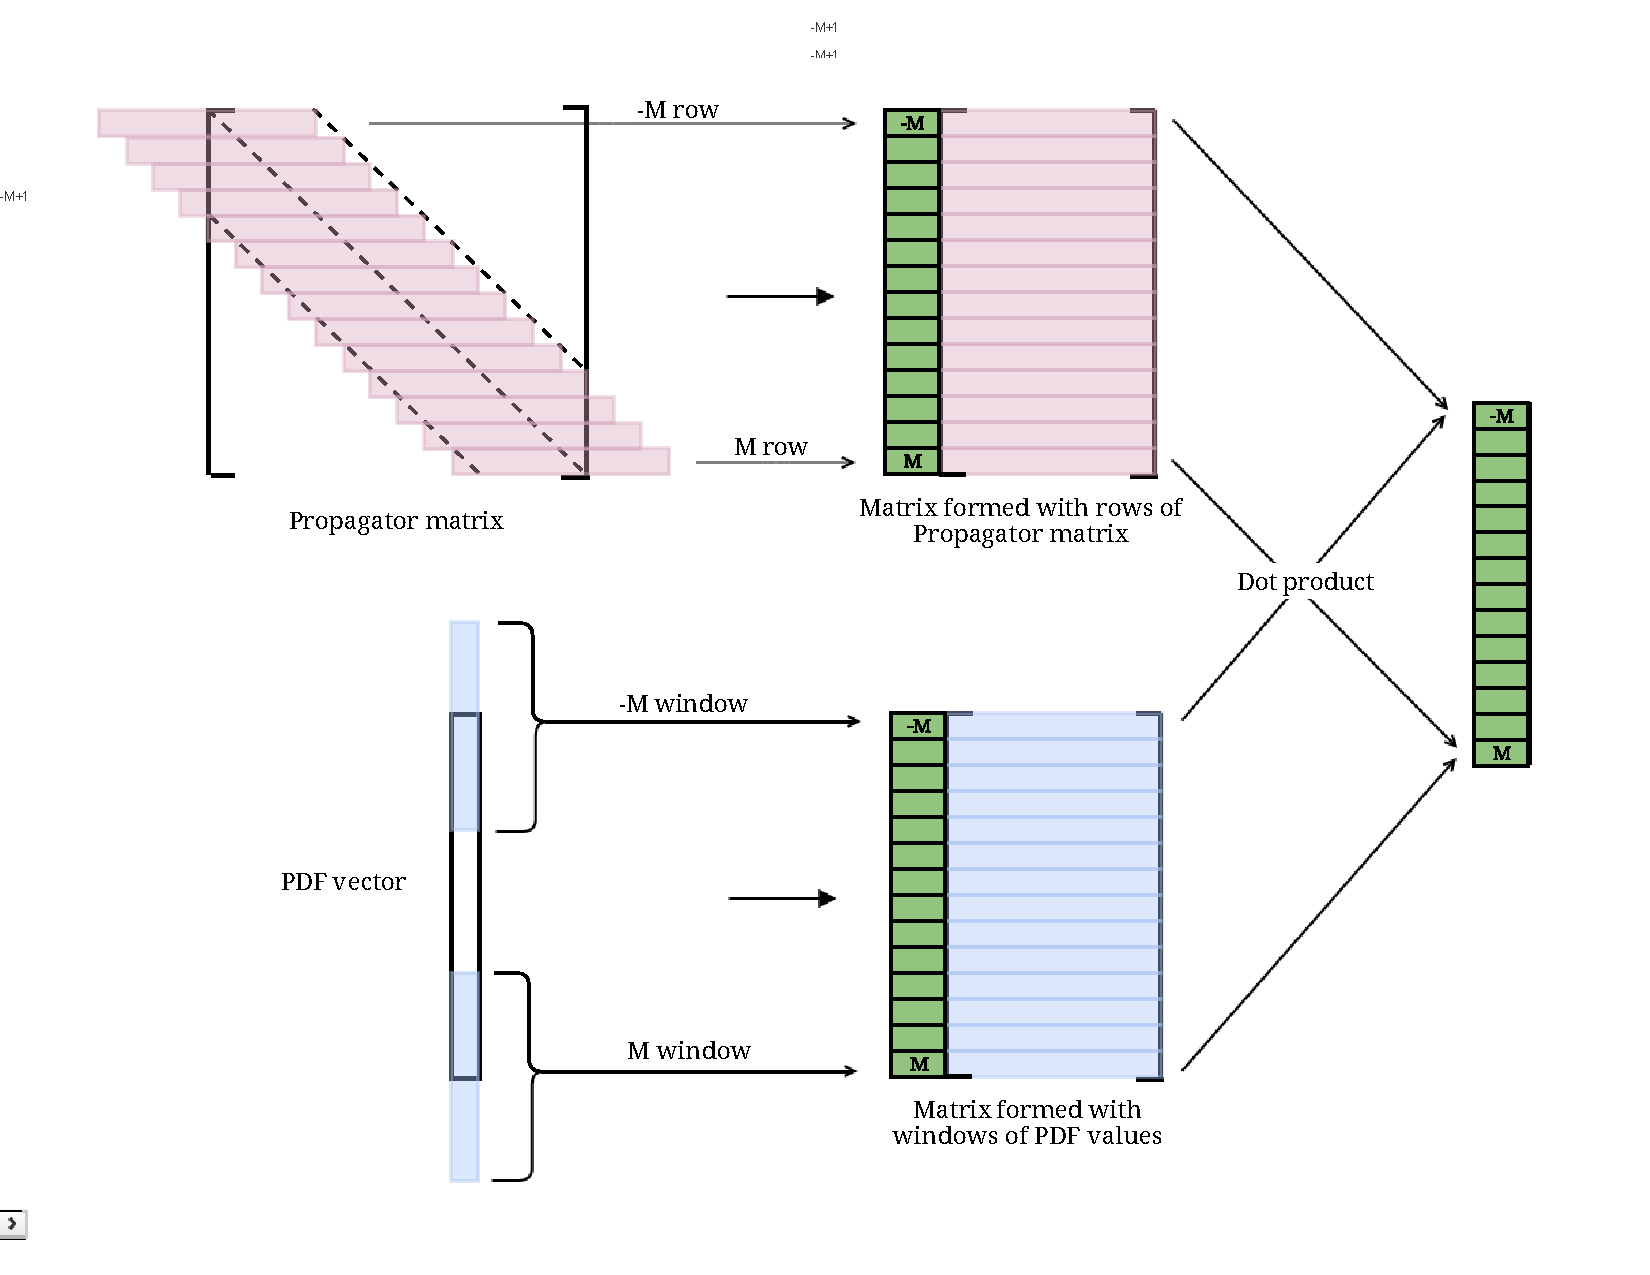
\includegraphics[width=6in]{gammawindow}
\end{center}
\caption{Making use of Scala, Breeze, and Intel MKL.}
\label{fig:implementation1}
\end{figure}



\section{Results}
We begin with results on artificial data sets.  The model used to
generate these data sets is the Ornstein-Uhlenbeck SDE
\begin{equation}
\label{eqn:ou}
{d}X_t = \theta_1 (\theta_2 - X_t) {d}t + \theta_3 {d}W_t
\end{equation}
together with the observation process
\begin{equation}
\label{eqn:ou_obs}
Y_t = X_t + \epsilon_t.
\end{equation}
Specifically, what we do is apply the Euler-Maruyama discretization to
(\ref{eqn:ou}) with a time step of $\kappa = 10^{-6}$.  Suppose our
temporal grid consists of $t_j = n(j) \kappa$, where $n(0) = 0$,
and $n(j+1) > n(j)$.  In some of the examples we pursue, $n(j)$ will
be deterministic and the temporal grid will be equispaced, while in other examples, $n(j)$ will
be stochastic and the temporal grid will be non-equispaced.  Either
way, we take $n(j)$ to have expected value $2 \times 10^5$, so that
the average difference between temporal grid points $t_{j+1} - t_j$ is $0.2$.

We then start at a
random initial condition by sampling $X_0$ from a Gaussian random
variable with mean $0$ and variance $1$.  We step forward one step at
a time (with time step $\kappa$), saving the numerical solution $X_t$
at points in time corresponding to the temporal grid points $\{t_j\}_{j=0}^M$.
We label the points we save as $(x_0, x_1, \ldots, x_M) =:
\mathbf{x}$, and then perturb them via (\ref{eqn:ou_obs}) to generate
$\mathbf{y}$.  In particular, we set $y_j = x_j + Z$ where $Z$ is
normally distributed with mean $0$ and variance $\sigma^2$.

The DTQ method described in Section \ref{sect:likelihood} has four
internal parameters: the time step $h$, the spatial grid spacing $k$,
the spatial grid cutoff $M$, and the decay width $\gamma$ of the Gaussian
kernel $G$.  For the tests described below, we will give the value of
$h$ that was used.  All other parameters are as follows: $k =
h^{0.75}$, $M = \lceil \pi/k^{1.5} \rceil$, and $\gamma = 25$.

\subsection{Equispaced Time Series}
\label{sect:equispaced}
In the first set of experiments, we follow the procedure outlined
above to generate artificial data $\mathbf{y}$ with the temporal grid
defined by $t_j = n(j) \kappa = (0.2) j$.  The ground truth for the
parameters consists of $\theta = (0.5, 1, 0.25)$ and $\sigma^2 =
0.01$.  In addition to the other parameters, we
focus on inferring $\theta_1$ and $\theta_2$; we fix $\theta_3 =
0.25$ throughout.  In the Metropolis algorithm, we take as initial conditions
$\mathbf{x}_0 = \mathbf{y}$, $\theta = (1,0.1,0.25)$, and
$\sigma_\epsilon^2 = 1$.

For priors for $\theta_1$ and $\theta_2$, we use Gaussian densities
with respective parameters $(\mu=0.5,\sigma=1)$ and
$(\mu=2,\sigma=10)$.  For $\sigma_\epsilon^2$, we use an exponential
prior with parameter $\lambda=1$.

In the Metropolis algorithm, we take all proposal random variables to
be independent Gaussians.  In particular, $Z_\mathbf{x}$ is a collection of
$M+1$ independent Gaussians, each with parameters
$(\mu=0,\sigma=0.02)$, $Z_\theta$ consists of two independent
Gaussians, each with parameters $(\mu=0,\sigma=0.05)$, and $Z_\sigma$
consists of a Gaussian with parameters $(\mu=0,\sigma=0.02)$.

For two values of the DTQ internal time step ($h = 0.02$ and
$h=0.01$), we apply the Metropolis algorithm to generate $10,000$
samples of the posterior (\ref{eqn:post2}).  

We discard the first $100$ samples as burn-in samples, i.e., samples
that are taken before the Metropolis Markov chain has reached
equilibrium.

\begin{figure}[th]
\begin{center}
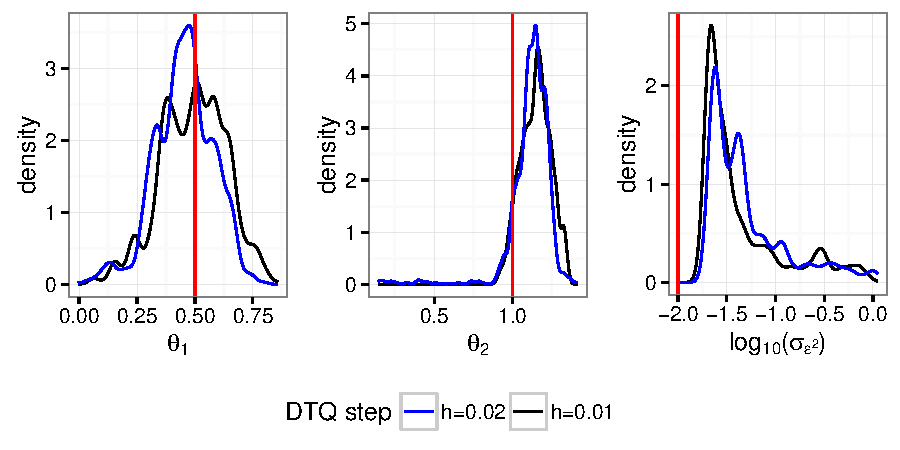
\includegraphics[width=6in]{post_equi}
\end{center}
\caption{Posterior densities for equispaced time series}
\label{fig:post_equi}
\end{figure}

\subsection{Non-equispaced Time Series}
\label{sect:nonequispaced}
In this next set of experiments, we follow a nearly identical
procedure to that described in Section \ref{sect:equispaced}.  The
main difference is that the temporal grid is defined by $t_j = n(j)
\kappa$ where $n(j)$ is uniformly distributed on the integers between
$4 \times 10^{4}$ and $4 \times 10^5 - 4 \times 10^4$.  Effectively,
this generates a time series with minimum, mean, and maximum spacings
$t_{j+1} - t_j$ of, respectively, $0.04$, $0.2$, and $0.36$.

\begin{figure}[th]
\begin{center}
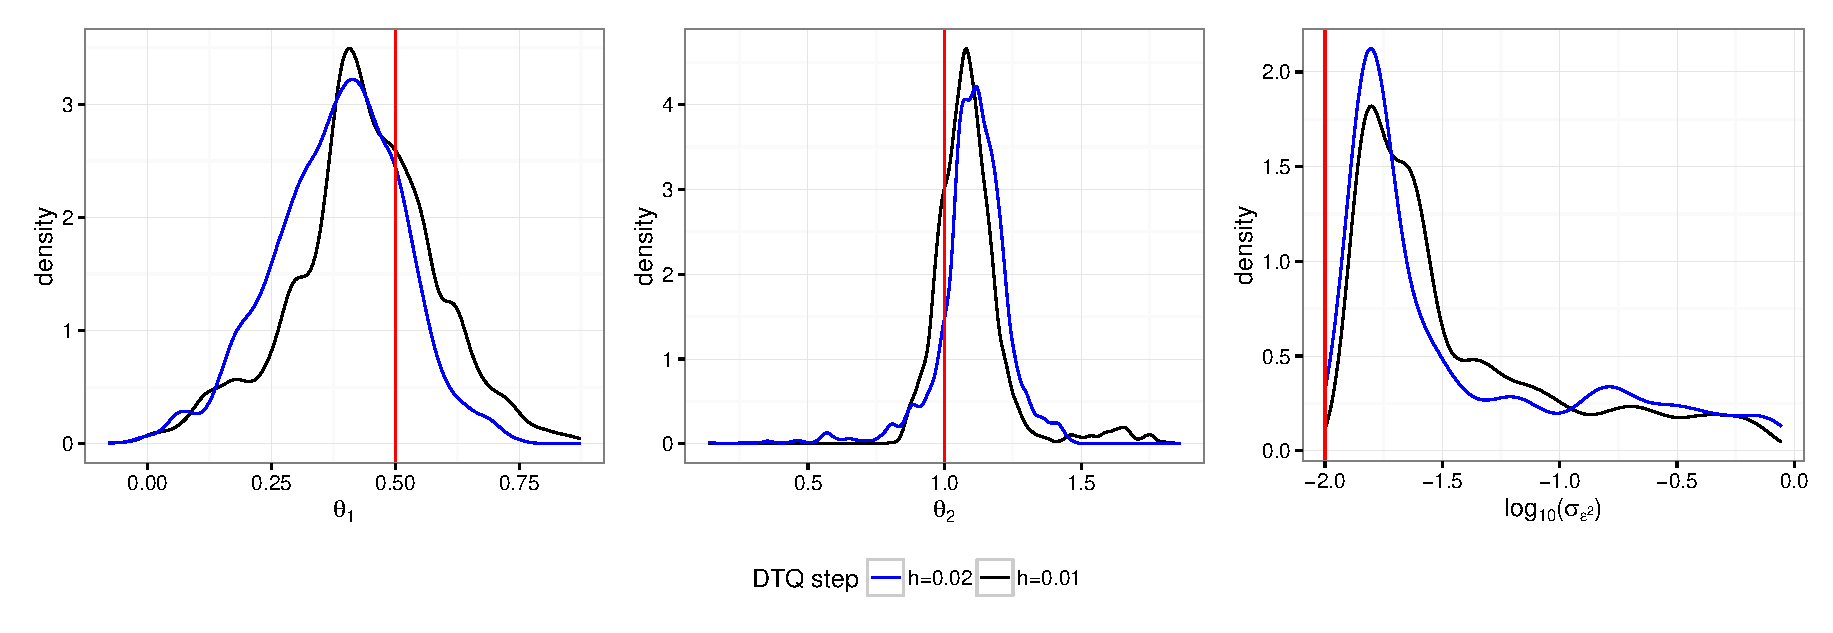
\includegraphics[width=6in]{post_nonequi}
\end{center}
\caption{Posterior densities for non-equispaced time series}
\label{fig:post_nonequi}
\end{figure}

\begin{figure}[th]
\begin{center}
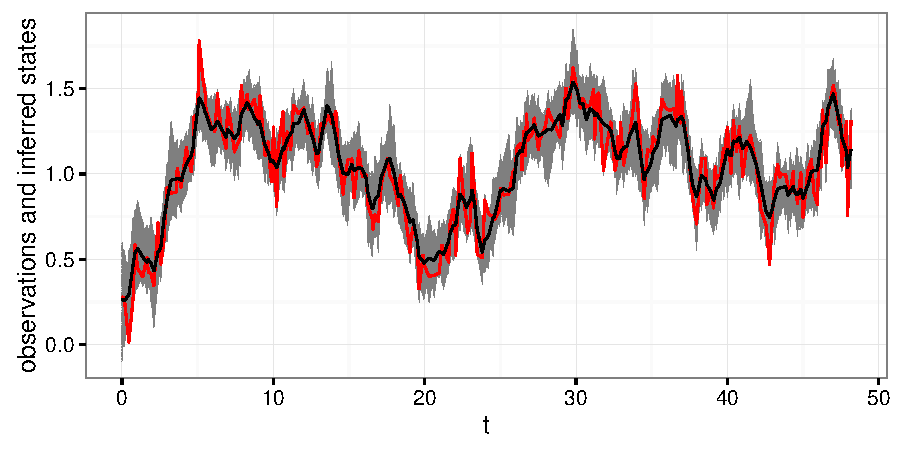
\includegraphics[width=6in]{timeseries1}
\end{center}
\caption{Observations and inferred states}
\label{fig:timeseries1}
\end{figure}

\begin{figure}[th]
\begin{center}
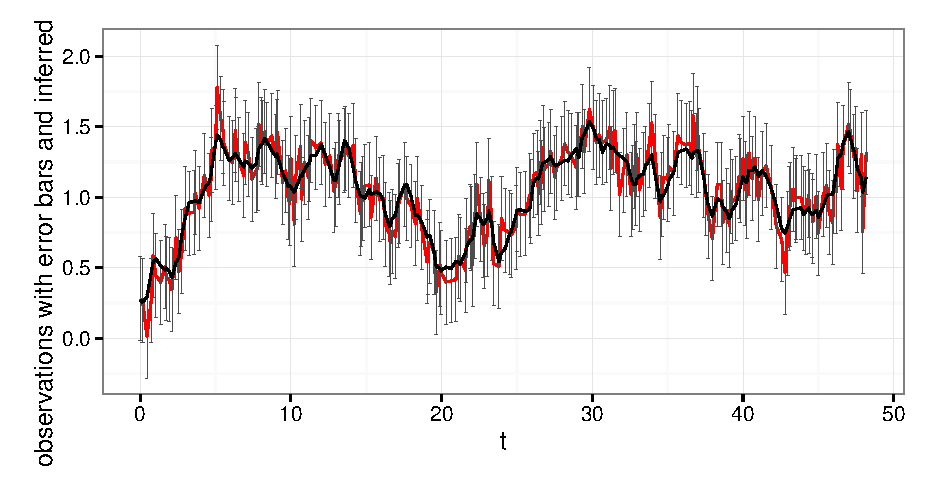
\includegraphics[width=6in]{timeseries2}
\end{center}
\caption{Observations and mean inferred state with error bars.  The
  error bars are computed by
  adding/subtracting the mean inferred value of $\sigma_\epsilon$ to
  the observation series $\mathbf{y}$.}
\label{fig:timeseries2}
\end{figure}

% first set of tests: determinstic tvec
% actual_bigrun1 and actual_bigrun2
% theta = 

% second set of tests: random tvec
% actual_bigrun7 and actual_bigrun6
% theta = (0.5, 1, 0.25) is true vec
% h = 0.01
% h = 0.02

\section{Conclusion}

\acks{This work was partially supported by a grant from UC Merced's
  Committee on Research (awarded to H.S. Bhat) and by UC Merced USAP fellowships
  (awarded to R.W.M.A. Madushani and S. Rawat).}

\bibliography{BhatMaduRawatBigMine16}

\end{document}

%%% Local Variables:
%%% mode: latex
%%% TeX-master: t
%%% End:
